\documentclass[Ex4_Zusammenfassung.tex]{subfiles}


\begin{document}

\chapter{Teilchendetektoren}
\textbf{Heinstein,Martina} \newline
Teilchendetektoren messen Produkte von Kollisionen und Zerfällen.

\subsubsection*{Aufgaben}
\begin{itemize}
	\item Nachweis entstandener Teilchen
	\item Messung von Energie/Impuls
	\item Messung von Lebensdauer, Zerfallslänge, $\beta,\ \gamma,\ \tau$
	\item Teilchenidentifikation (Bestimmung $M^2 = E^2 - \vec{p}^2$)
\end{itemize}

\subsubsection*{Kapitel}
\begin{enumerate}[\hspace{0.5cm}{4.}1]
\item Impulsmessung
\item Energiemessung
\item Messung von Photonen
\item Teilchen
\end{enumerate}

\section{Impulsmessung}
Ablenkung von geladenen Teilchen im Magnetfeld.\\
$\rightarrow$ Homogenes B-Feld\\
$\rightarrow$ Kreisbahn mit Radius $r=\frac{p}{q\cdot B}$

\subsection*{Gasdetektor}
\begin{itemize}
	\item Kondensator $\rightarrow$ E-Feld
	\item Ionisationsgas, nicht elektronegativ\\ $\Delta U = -\frac{N\cdot e }{C}$, wobei $N$ die Teilchenanzahl, $e$ die Elementarladung und $C$ die Kapazität des Kondensators ist. ( siehe Abb. ~\ref{Gasdetektor} )
\end{itemize}

\begin{figure}[H]
	\centering
	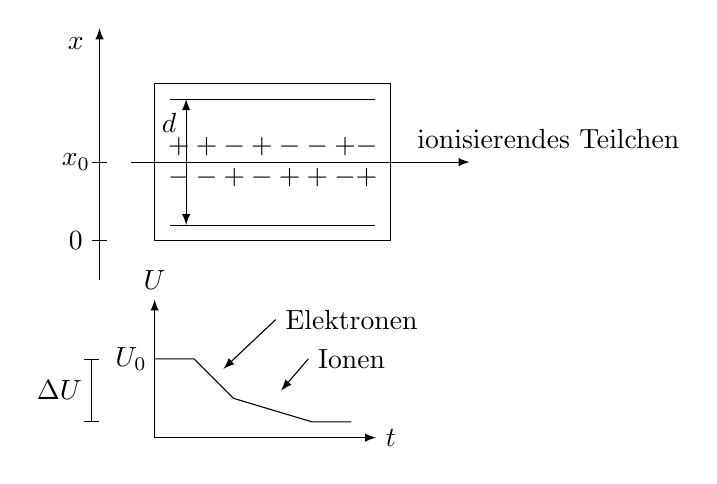
\begin{tikzpicture}
		\node at (0,0) (x0) {$x_0$};
		\node at (0,1.5) (x) {$x$};
		\node at (0,-1) (null) {$0$};
		\node at (6,0.3) (teilchen) {ionisierendes Teilchen};
		\node at (2.5, 0.2) (ladung1) {$++-+--+-$};
		\node at (2.5, -0.2) (ladung2) {$--+-++-+$};
		
		\draw [->, >=latex, thin] (0.3, -1.5) -- (0.3, 1.7);
		\draw [->, >=latex, thin] (0.7,0) -- (5,0);
		\draw (0.2,-1) -- (0.4,-1);
		\draw (0.2,0) -- (0.4, 0);
		\draw (1,-1) -- (4,-1) -- (4,1) -- (1,1) -- cycle;
		\draw (1.2, -0.8) -- (3.8, -0.8);
		\draw (1.2, 0.8) -- (3.8, 0.8);
		\draw [<->, >=latex] (1.4, -0.8) -- (1.4, 0.8) node [pos=0.5,anchor=east,yshift=0.5cm] {$d$};
		%%
		% Diagramm:
		%%
		\node at (1, -1.5) (U) {$U$};
		\node at (4, -3.5) (t) {$t$};
		\node at (0.7, -2.5) (U0) {$U_0$};
		\node at (3.5, -2) (Elektronen) {Elektronen};
		\node at (3.5, -2.5) (Ionen) {Ionen};
		
		\draw [<->, >=latex] (U) -- (1, -3.5) -- (t);
		\draw (1,-2.5) -- (1.5, -2.5) -- (2, -3) node [midway, above] (elek) {} -- (3,-3.3) node [midway, above] (ions) {} -- (3.5, -3.3);
		\draw [->, >=latex] (Elektronen.west) -- (elek.east);
		\draw [->, >=latex] (Ionen.west) -- (ions);
		\draw [|-|] (0.2,-2.5) -- (0.2, -3.3) node [pos=0.5, anchor=east] {$\Delta U$};
		
	\end{tikzpicture}
	\caption{Schematischer Aufbau eines Gasdetektors (oben) \\ Spannungsänderung am Kondensator über Zeit (unten)}\label{Gasdetektor}
\end{figure}

\subsection*{Proportionalzählrohr}
\begin{itemize}
	\item sehr dünner Anodendraht  $ \rightarrow  \si{$ \mu {m} $} $ 
	\item $E(r) = \frac{U_0}{r \cdot \ln \left| \frac{R}{r_A} \right|} \Rightarrow$ starkes Feld im Zentrum (siehe Abb.~\ref{Proportionalzaehlrohr} )
	\item \textbf{Sau} starke Beschleunigung in Nähe des Anodendrahtes
	\item Reicht aus, im Gas zu ionisieren $\rightarrow$ Sekundärelektronen\\
		$\Delta U = - \frac{ANe}{C}, \quad A=10^4 - 10^5$ Verstärkungsfaktor
	
\end{itemize}

\begin{figure}[H]
	\centering
	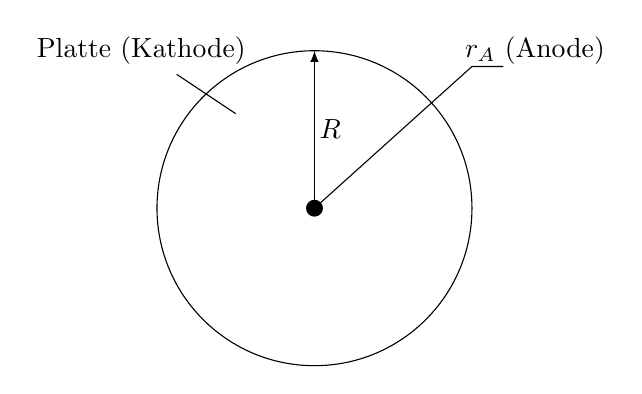
\begin{tikzpicture}
		\node at (-2.2, 2) (Platte) {Platte (Kathode)};
		
		\draw (0,0) circle (2cm);
		\draw [fill=black] (0,0) circle (0.1cm);
		\draw [->, >=latex] (0,0) -- (0,2) node [midway, xshift=0.2cm] (R) {$R$};
		\draw (0,0) -- (2,1.8) -- (2.4, 1.8) node [at end, yshift=0.2cm, xshift=0.4cm] (rA) {$r_A$ (Anode)};
		\draw (Platte) -- (-1.0, 1.2);
	\end{tikzpicture}
	\caption{Schema eines Proportionalzählrohrs}\label{Proportionalzaehlrohr}
	
\end{figure}

\subsection*{Halbleiterzähler}
Ein Halbleiterzähler ist ein pn-Übergang, an den in Sperrrichtung eine Spannung angelegt wird. Dadurch entsteht eine Verarmungszone, in der keine freien Ladungsträger vorhanden sind.\\
Durchgehende Teilchen erzeugen durch Ionisation in dieser Zone Elektronen-Loch-Paare, die im E-Feld zu den Anschlusspolen wandern und ein Signal erzeugen. 

\subsection*{Szintillationszähler}
\begin{itemize}
	\item Teilchen oder $\gamma$-Teilchen gibt Energie ab, die in Form von sichtbarem Sicht wieder frei wird.
	\item Auslesen durch Photodetektor
\end{itemize}

\section{Energiemessung}

\begin{itemize}
	\item Absorbtion eines hadronischen Schauers in Kaloriemeter
	\item \boxed{\text{Hadronen: z.B. Protonen, Neutronen.. (aus Quarks zusammengesetzte Teilchen)}}
\end{itemize}

\subsection*{hadronischer Schauer}
Beim Einfall hochenergetischer Teilchen entstehen Sekundärteilchen, die selbst so lange Teilchen generieren, bis die Energie erschöpft ist. \\

\textbf{Beispiel:}\\
Mittlere Weglänge eines Teilchens in Blei: $5.6 \si{mm} = \lambda$\\
Ideale Länge: $20 \lambda \rightarrow 112 \si{mm}$ Blei\\
Abwechselnd: $2 \si{mm}$ Blei und  $5 \si{mm}$ Szintillationszähler\\
$\rightarrow 392 \si{mm}$ Länge (elektromagnetisches Kaloriemeter, ECAL)\\

Hadronen: Absorbtionslänge $\lambda = 18.5 \si{cm} \rightarrow 10 \lambda = 1.85 \si{m}+$ECAL

\subsection{Messung von Photonen}
\begin{itemize}
	\item Röntgen- \& Gammastrahlen in Halbleiterkristallen (Si, Ge, ...) $\rightarrow$ gute Auflösung
	\item Messung durch szintillierende Kristalle ($NaT, PbWO_4$)
		\begin{itemize}
			\item niedrige Energie $\rightarrow$ schlechte Auflösung
			\item hohe Energie ($>100 \si{MeV}$)+ ausreichende Dichte $\rightarrow$ gute Messung
			\item ''Kristallkaloriemeter'': $\frac{\sigma_E}{E} = \frac{0.04}{\sqrt{E}} + 0.01 
				\begin{cases}
					\text{für }1 \si{GeV}&: \frac{\sigma_E}{E}=4.1\% \\
					\text{für }100 \si{GeV} &: \frac{\sigma_E}{E} = 1.1\%
				\end{cases}$
		\end{itemize}
\end{itemize}

\section{Teilchenidentifikation}
\begin{itemize}
	\item Massenbestimmung durch Messung von Impuls \& Flugzeit\\
		$pc = \beta E = \beta \gamma m_0 c^2$\\
		Impulsbereich limitiert durch Auflösung von Zeitmessung \& Flugstrecken\\
		Grenze der Methode: Impuls etwa in $\frac{\si{GeV}}{c}$
	\item Massenbestimmung durch Zerfallsprodukte (Masse \& Impulse erhalten!)\\
		$K^0 \rightarrow \pi^+ \pi^-$
	\item durch spezifische Energieverluste\\
		Bei bekanntem $p\cdot c$ wird $\frac{\md E}{\md x}$ gemessen $\rightarrow \beta \gamma$ bestimmt
	\item durch ''Tricks'':
		\begin{itemize}
			\item Myonen: nur Energieverluste durch Ionisation, keine Schauer
			\item Photonen: keine Energieverluste durch Ionisation, nur el.mag. Schauer
			\item Elektronen: Energieverluste durch Ionisation, el.mag. Schauer, Übergangsstrahlung
			\item Neutronen, Antineutronen: keine Ionisation, nur hadronischer Schauer
			\item geladene, hochenergetische Teilchen: Cherenkov-Strahlung (Teilchen in Medium schneller als Licht $\rightarrow$ strahlen Licht ab (Energie ändert sich nicht wirklich) über welches Information über Teilchen zu erhalten sind.)
		\end{itemize} 
\end{itemize}
\end{document}